\documentclass[10pt]{article}
\usepackage[utf8]{inputenc}
\usepackage[T1]{fontenc}
\usepackage{amsmath}
\usepackage{amsfonts}
\usepackage{amssymb}
\usepackage{mhchem}
\usepackage{stmaryrd}
\usepackage{bbold}
\usepackage{graphicx}
\usepackage[export]{adjustbox}
\graphicspath{ {./images/} }

\title{Ph.D. Qualifying Exam in Analysis, by Paul Muhly and Lihe Wang }

\author{}
\date{}


\begin{document}
\maketitle
\section{Qualifying Exam -Analysis 
 Summer 2020}
Professors Ionut Chifan and Lihe Wang

\section{Rules of the exam}
\begin{itemize}
  \item You have 180 minutes to complete this exam.

  \item The exam contains a section of 5 problems in real analysis and a section of 5 problems in complex analysis. For maximum points you must submit solutions for 7 problems, at least 3 from each section.

  \item Please mark the problems to be graded on the first column of the grading table on page $2 .$

  \item Show your work! - any answer without an explanation will get you zero points.

  \item Please read the questions carefully; some ask for more than one thing.

  \item Do not forget to write your name, see page 2 .

  \item You are not allowed to use a calculator, cell phone, ipad or any other internet browser device during the exam.

\end{itemize}
\section{Good luck!}
NAME (PRINT):

Mark in the first column below which problems should be graded!

\begin{tabular}{|l|c|c|c|}
\hline
Your Choice & Problem & Points & Your Score \\
\hline
 & R - I & 25 & $\mid$ \\
\hline
 & R - II & 25 & $\mid$ \\
\hline
 & R - III & 25 &  \\
\hline
 & R - IV & 25 &  \\
\hline
 & R - V & 25 &  \\
\hline
 & C - I & 25 &  \\
\hline
 & Cotal & 175 &  \\
\hline
 & C - II & 25 &  \\
\hline
 & C - IV & 25 &  \\
\hline
 & C II & 25 &  \\
\hline
 &  &  &  \\
\hline
 &  &  &  \\
\hline
 &  &  &  \\
\hline
 &  &  &  \\
\hline
 &  &  &  \\
\hline
\end{tabular}

\section{Real Analysis}
$\mathbf{R}$ - I: Solve at your choice ONE of the following problems:

a) Suppose for all any $x \in(0,1)$ and $\varepsilon>0$ there exists $0<r<\varepsilon$, such that $\int_{x-r}^{x+r} f(x) d x \geq 2 r$. Show that $f \geq 1$ a.e for $x \in[0,1]$.

b) Is there a closed, uncountable subset of $\mathbb{R}$ containing no rational numbers? Justify your answer!

c) (True-False) Let $f: \mathbb{R} \rightarrow \mathbb{R}$ be a measurable function and denote by $A=\left\{x \in \mathbb{R}: m\left(f^{-1}(\{x\})\right)>0\right\}$. Then $m(A)=0$. If you believe is true provide a proof otherwise supply a counterexample.

$\mathbf{R}$ - II: (True-False) If $f$ is integrable on $\mathbb{R}$ then $\lim _{x \rightarrow \infty} f(x)=0$. If you believe it is true provide a proof, otherwise supply a counterexample.

R - III: Suppose $E$ is a measurable set such that $m(E \cap(a, b)) \geq \frac{b-a}{2}$ for all $a<b$. Show that $E$ is the whole axis except a measure zero set.

$\mathbf{R}$ - IV: Let $A$ be a measurable subset of $[0,2]$ and define $f: \mathbb{R} \rightarrow \mathbb{R}$ by letting $f(x)=m((-\infty, x] \cap A)$, for every $x \in \mathbb{R}$; here $m$ is the Lebesgue measure on $\mathbb{R}$.

1.) Show that $f$ is absolutely continuous on $\mathbb{R}$, calculate $f^{\prime}$ and $\int_{0}^{3} f^{\prime}(x) d m(x)$, explaining your reasoning.

2.) Show that for every $0<b<m(A)$ there exists $x_{0} \in \mathbb{R}$ such that $b=m\left(\left(-\infty, x_{0}\right] \cap A\right)$.

Make sure you state correctly all the results you use in the proof.

$\mathbf{R}$ - V: Let $1 \leq p<\infty$ and suppose that $f, f_{k} \in L^{p}(\mathbb{R})$ are functions satisfying $\lim _{k \rightarrow \infty} f_{k}(x)=f(x)$, for almost every $x \in \mathbb{R}$. Then prove that $\lim _{k \rightarrow \infty}\left\|f_{k}-f\right\|_{L^{p}}=0$ if and only if $\lim _{k \rightarrow \infty}\left\|f_{k}\right\|_{L^{p}}=\|f\|_{L^{p}}$.

\section{Complex analysis}
C - I: Solve at your choice ONE of the following problems:

a) If $0<a<1$ then show that
$$
\int_{-\infty}^{\infty} \frac{e^{a x}}{1+e^{x}} d x=\frac{\pi}{\sin (a \pi)}
$$
b) (True-False) Let $f$ be analytic on the open punctured unit disk $D(0,1) \backslash\{0\}$. Can $f^{\prime}$ have a polar singularity of order one at 0 ? If you believe it is true provide a proof, if not supply a counterexample. Also make sure you include all the details in your arguments.

c) Assume that $\left(a_{n}\right)=(1,1,2,3,5,8, \ldots)$ is Fibonacci sequence. Consider the power series $f(z)=$ $\sum_{n} a_{n} z^{n}$. Find the radius of convergence for $f(z)$ and determine a singularity point of the circle of convergence in case it is finite.

$\mathbf{C}$ - II: Find all entire functions $f$ of finite order such that $f$ has 2020 roots and $f^{\prime}$ has 2022 roots, counted with their multiplicities. State clearly all the theorems you are using.

$\mathbf{C}$ - III: Assume that $f$ is an entire function such that $|f(z)|=1$ when $|z|=1$. Prove that $f(z)=a z^{n}$ for some integer $n \geq 0$ and some $a \in \mathbb{C}$ with $|a|=1$.

$\mathbf{C}$ - IV: Let $\mathcal{F}$ be the class of all $f \in H(D(0,1))$ such that $\operatorname{Re} f>0$ and $f(0)=1$. Show $\mathcal{F}$ is a normal family.

$\mathbf{C}$ - V: Suppose that $f: D(0,1) \rightarrow P$ is a conformal mapping onto a regular pentagonal region $P$, with center at 0 such that $f(0)=0$. Compute $f^{(2020)}(0)$.

(Here we denoted by $f^{(n)}$ the $n$-th derivative of $f$.) $\mathbf{R}$ - I:Solve at your choice ONE of the following problems:

a) Suppose for all any $x \in(0,1)$ and $\varepsilon>0$ there exists $0<r<\varepsilon$, such that $\int_{x-r}^{x+r} f(x) d x \geq 2 r$. Show that $f \geq 1$ a.e for $x \in[0,1]$.

b) Is there a closed, uncountable subset of $\mathbb{R}$ containing no rational numbers? Justify your answer!

c) (True-False) Let $f: \mathbb{R} \rightarrow \mathbb{R}$ be a measurable function and denote by $A=\left\{x \in \mathbb{R}: m\left(f^{-1}(\{x\})\right)>0\right\}$. Then $m(A)=0$. If you believe is true provide a proof, otherwise supply a counterexample.

Make sure you state correctly all the results you use in the proof.

Solution: PROBLEM: R - II:(True-False) If $f$ is integrable on $\mathbb{R}$ then $\lim _{x \rightarrow \infty} f(x)=0$. If you believe it is true provide a proof, otherwise supply a counterexample.

Make sure you state correctly all the results you use in the proof.

\section{Solution:}
PROBLEM: R - III: Suppose $E$ is a measurable set such that $m(E \cap(a, b)) \geq \frac{b-a}{2}$ for all $a<b$. Show that $E$ is the whole axis except a measure zero set.

Make sure you state correctly all the results you use in the proof.

Solution: PROBLEM: $\mathbf{R}$ - IV: Let $A$ be a measurable subset of $[0,2]$ and $\operatorname{define} f: \mathbb{R} \rightarrow \mathbb{R}$ by letting $f(x)=$ $m((-\infty, x] \cap A)$, for every $x \in \mathbb{R}$; here $m$ is the Lebesgue measure on $\mathbb{R}$.

1.) Show that $f$ is absolutely continuous on $\mathbb{R}$, calculate $f^{\prime}$ and $\int_{0}^{3} f^{\prime}(x) d m(x)$, explaining your reasoning.

2.) Show that for every $0<b<m(A)$ there exists $x_{0} \in \mathbb{R}$ such that $b=m\left(\left(-\infty, x_{0}\right] \cap A\right)$.

Make sure you state correctly all the theorems you use in the proof.

Solution: PROBLEM: $\mathbf{R}-\mathbf{V}:$ Let $1 \leq p<\infty$ and suppose that $f, f_{k} \in L^{p}(\mathbb{R})$ are functions satisfying lim $k \rightarrow \infty f_{k}(x)=$ $f(x)$, for almost every $x \in \mathbb{R}$. Then prove that $\lim _{k \rightarrow \infty}\left\|f_{k}-f\right\|_{L^{p}}=0$ if and only if $\lim _{k \rightarrow \infty}\left\|f_{k}\right\|_{L^{p}}=\|f\|_{L^{p}}$. Make sure you state correctly all the theorems you use in the proof.

Solution: PROBLEM: C - I: Solve at your choice ONE of the following problems:

a) If $0<a<1$ then show that
$$
\int_{-\infty}^{\infty} \frac{e^{a x}}{1+e^{x}} d x=\frac{\pi}{\sin (a \pi)}
$$
b) (True-False) Let $f$ be analytic on the open punctured unit disk $D(0,1) \backslash\{0\}$. Can $f^{\prime}$ have a polar singularity of order one at 0? If you believe it is true provide a proof, if not supply a counterexample. Also make sure you include all the details in your arguments.

c) Assume that $\left(a_{n}\right)=(1,1,2,3,5,8, \ldots)$ is Fibonacci sequence. Consider the power series $f(z)=$ $\sum_{n} a_{n} z^{n}$. Find the radius of convergence for $f(z)$ and determine a singularity point of the circle of convergence in case it is finite.

Make sure you state correctly all the results you use in the proof.

Solution: PROBLEM: C - II. Find all entire functions $f$ of finite order such that $f$ has 2020 roots and $f^{\prime}$ has 2022 roots, counted with their multiplicities. State clearly all the theorems you are using.

Make sure you state correctly all the results you use in the proof.

\section{Solution:}
PROBLEM: C - III. Assume that $f$ is an entire function such that $|f(z)|=1$ when $|z|=1$. Prove that $f(z)=a z^{n}$ for some integer $n \geq 0$ and some $a \in \mathbb{C}$ with $|a|=1$.

Make sure you state correctly all the results you use in the proof.

\section{Solution:}
PROBLEM: C - IV. Let $\mathcal{F}$ be the class of all $f \in H(D(0,1))$ such that $R e f>0$ and $f(0)=1$. Show $\mathcal{F}$ is a normal family.

Make sure you state correctly all the results you use in the proof.

Solution: PROBLEM: C - V. Suppose that $f: D(0,1) \rightarrow P$ is a conformal mapping onto a regular pentagonal region $P$, with center at 0 such that $f(0)=0$. Compute $f^{(2020)}(0)$.

(Here we denoted by $f^{(n)}$ the $n$-th derivative of $f$.)

Make sure you state correctly all the results you use in the proof.

Solution:

\section{Ph.D. Qualifying Examination in Analysis}
Professors Ionut Chifan and Paul Muhly

August 15, 2018

Instructions. Be sure to put your name on each booklet you use.

This examination has a number of "true-false" questions in it. When a problem is a true-false problem, the operative statement will be preceded by True-False?. You are to decide whether it is true or false. If you think it is true, you must provide a proof. If you think it is false, you must provide a counter example or a proof of why it is false. No points will be given for a correct guess that the problem is true or false without any justification. Also, there will be no "Bankruptcy" points given.

The exam is divided into two parts. The first covers real analysis and the second covers complex analysis. Each part has 5 problems. You need only work 4 problems in each part. You must indicate which 4 you are submitting for evaluation. If you want to do five in a part, that is OK. We will treat the extra problem as a bonus, but still mark the four problems (in each part) that you think are your best work.

\section{Part I}
\begin{enumerate}
  \item Let $f$ be a real-valued function defined on the interval $[0,1]$. True-False? If $f$ is not of bounded variation on $[0,1]$, then there is a point $x_{0}$ in $[0,1]$ such that on any open interval $I$ about $x_{0}, f$ fails to be of bounded variation on $I$.

  \item A (parametrized) curve $C$ in the plane is given by a pair of real-valued functions $f$ and $g$ defined on an interval $[a, b]$. (So as a point set, $C=\{(f(t), g(t)) \mid t \in[a, b]\}$.) The length of $C$ is defined to be

\end{enumerate}
$$
\sup \left\{\sum_{i=1}^{n}\left[\left(f\left(t_{i}\right)-f\left(t_{i-1}\right)\right)^{2}+\left(g\left(t_{i}\right)-g\left(t_{i-1}\right)\right)^{2}\right]^{\frac{1}{2}}\right\}
$$
where the sup is taken over all partitions $a=t_{0}<t_{1}<t_{2}<\cdots<t_{n-1}<t_{n}=b$. True-False? The length of $C$ is finite if and only if $f$ and $g$ are of bounded variation.

\begin{enumerate}
  \setcounter{enumi}{3}
  \item Let $\left\{U_{n}\right\}_{n=1}^{\infty}$ be a sequence of open sets in $[0,1]$. True-False? If the interior of $K:=\cap_{n=1}^{\infty} U_{n}$ is empty, then the Lebesgue measure of $K$ is zero.

  \item Let $f$ be a non-negative real-valued function defined on the interval $[0,1]$. True-False? $f$ is measurable if and only if there is a (finite or infinite) sequence $\left\{E_{n}\right\}$ of measurable subsets of $[0,1]$ and a sequence of non-negative constants $\left\{c_{n}\right\}$ such that $f(x)=\sum c_{n} 1_{E_{n}}(x)$ for every $x \in[0,1]$.

  \item Let $\left\{f_{n}\right\}_{n \geq 1}$ be a sequence of non-negative Lebesgue measurable functions defined on $\mathbb{R}$ that converges almost everywhere (with respect to Lebesgue measure $m$ ) to the function $f$. True-False? If $\lim _{n \rightarrow \infty} \int_{\mathbb{R}} f_{n} d m=0$, then $f=0$ a.e. with respect to $m$.

\end{enumerate}
\section{Part II}
\begin{enumerate}
  \setcounter{enumi}{6}
  \item Let $P_{n}(z):=\sum_{k=0}^{n-1}(k+1) z^{k}, n=1,2, \cdots$ and let $0<r<1$. True-False? There is an $n_{0}$ such that for all $n>n_{0}, P_{n}$ has no zero in the $\operatorname{disc}\{|z|<r\}$.

  \item Suppose $a$ is an isolated singularity of $f$ and suppose the real part of $f, \mathfrak{R}(f(z))$, satisfies the inequality $\mathfrak{R}(f(z)) \leq-m \ln |z-a|$ for some positive integer $m$ and for $z$ in some disc centered at $a$. What kind of singularity is $a$ ? (Is it removable, a pole, or essential?)

  \item Let $C$ be the circle $x^{2}+y^{2}=2 x$ oriented in the counter clockwise direction. Calculate $\int_{C} \frac{d z}{z^{4}+1}$.

  \item Let $\Omega$ be a region in the plain, $\mathbb{C}$, and let $\mathcal{F}_{\Omega}=\cup_{n \geq 0}\left\{f|f| \Omega=z^{n}\right\}$. Identify all the regions $\Omega$ such that $\mathcal{F}_{\Omega}$ is a normal family. 10. Suppose the series $\sum_{k=0}^{\infty} b_{n} z^{n}$ converges in the open unit disc and that $b_{n} \geq 0$ for all $n$. Let

\end{enumerate}
$$
\mathcal{F}=\left\{\sum_{k=0}^{\infty} a_{n} z^{n}|| a_{n} \mid \leq b_{n}\right\}
$$
True-False? $\mathcal{F}$ is a normal family.

\section{Qualifying Exam -Analysis 
 Winter 2018}
Professors Ionut Chifan and Paul Muhly

\section{Rules of the exam}
\begin{itemize}
  \item You have 180 minutes to complete this exam.

  \item The exam contains a section of 4 problems in real analysis and a section of 4 problems in complex analysis. For maximum points you must submit solutions for 6 problems. Also you must attempt at least 2 problems in each section.

  \item Please mark the problems to be graded on the first column of the grading table on page $2 .$

  \item Show your work! - any answer without an explanation will get you zero points.

  \item Please read the questions carefully; some ask for more than one thing.

  \item Do not forget to write your name, see page 2 .

  \item You are not allowed to use a cell phone or a calculator during the exam.

\end{itemize}
\section{Real Analysis}
$\mathbf{R}$ - I: Solve at your choice ONE of the following problems:

a) Let $E \subseteq \mathbb{R}$ be a Lebesgue measurable set such that $3 \mu(E \cap(a, b)) \leq b-a$ for all $a<b$. Find $\mu(E)$. Make sure you include all the details in your arguments.

b) Let $f: \mathbb{R} \rightarrow \mathbb{R}$ be an increasing function. Show that $f$ has at most countably many discontinuity points. Conversely, if $A \subset \mathbb{R}$ is a countable subset then there exists a increasing function $f$ whose discontinuity points coincide with $A$. Make sure you include all the details in your arguments.

$\mathbf{R}$ - II: Let $p \geq 1$. Assume that $\mathrm{f}$ is an absolute continuous function on any compact interval and moreover $f^{\prime} \in L^{p}(\mathbb{R}, \mu)$. Show that
$$
\sum_{n \in \mathbb{Z}}|f(n+1)-f(n)|^{p}<\infty .
$$
$\mathbf{R}$ - III: Let $(X, d)$ be a compact metric space and let $f: X \rightarrow X$ be an isometry (i.e. $d(f(x), f(y))=d(x, y)$ for all $x, y \in X$ ). Show that $f$ is a homeomorphism (i.e. it is continuous, invertible, and the inverse is continuous as well).

$\mathbf{R}$ - IV: Let $f_{n} \in L^{3}((0,1))$ nonnegative functions such that $\left\|f_{n}\right\|_{3}=1$ for all $n$ and $f_{n} \rightarrow 0$ almost everywhere as $n \rightarrow \infty$. Show that $\int_{0}^{1} f_{n} d \mu \rightarrow 0$ as $n \rightarrow \infty$.

\section{Complex analysis}
$\mathbf{C}-\mathbf{I}$ : Solve at your choice ONE of the following problems:

a) Compute the following integral
$$
\int_{0}^{\infty} \frac{d x}{1+x^{7}}
$$
b) Construct a conformal map from the unit disk onto the infinite horizontal strip $|\operatorname{Im}(z)|<1$. Make sure you include all the details in your arguments.

c) TRUE-FALSE: Let $f$ be analytic on the open punctured unit disk $\mathbb{D} \backslash\{0\}$. Can $f^{\prime}$ have a polar singularity of order one at 0? Make sure you include all the details in your arguments.

$\mathbf{C}$ - II: Suppose $f: \mathbb{C} \backslash\{0\} \rightarrow \mathbb{R}$ is a nonconstant, real-valued harmonic function on the punctured plane. Prove that the image of $f$ is all of $\mathbb{R}$.

$\mathbf{C}$ - III: Suppose $f$ is a holomorphic function on $\{z \in \mathbb{C}|| z \mid<1\}$, the open unit disk, with the property that $\operatorname{Re} f(z)>0$ for every point $z$ in the disk. Prove that $\left|f^{\prime}(0)\right| \leq 2 \operatorname{Re} f(0)$.

$\mathbf{C}$ - IV: Let $f: \mathbb{C} \rightarrow \mathbb{C}$ be an injective holomorphic function. Show there exists $a, b \in \mathbb{C}$ such that $f(z)=a z+b .$

\section{Qualifying Exam -Analysis 
 Winter 2017}
Professors Ionut Chifan and Paul Muhly

\section{Rules of the exam}
\begin{itemize}
  \item You have 180 minutes to complete this exam.

  \item The exam contains a section of 5 problems in real analysis and a section of 5 problems in complex analysis. For maximum points you must submit solutions for 7 problems. Also you must attempt at least 2 problems in each section.

  \item Please mark the problems to be graded on the first column of the grading table on page 2 .

  \item Show your work! - any answer without an explanation will get you zero points.

  \item Please read the questions carefully; some ask for more than one thing.

  \item Do not forget to write your name, see page 2 .

  \item You are not allowed to use a cell phone or a calculator during the exam.

\end{itemize}
\section{Real Analysis}
$\mathbf{R}$ - I: Solve at your choice ONE of the following problems:

a) Let $E$ be a measurable set such that $0<\mu(E)<\infty$. Show that the set $E-E=\{x-y: x, y \in E\}$ contains an nonempty open interval.

b) Show that if $f: \mathbb{R} \rightarrow \mathbb{R}$ is measurable then the set $\left\{x \in \mathbb{R}: \mu\left(f^{-1}(x)\right)>0\right\}$ has measure zero.

$\mathbf{R}$ - II: Let $f: \mathbb{R} \rightarrow \mathbb{R}$ be Lebesque integrable on the real line. Show that
$$
\lim _{h \rightarrow 0} \int_{\mathbb{R}}|f(x+h)-f(x)| d \mu(x)=0
$$
$\mathbf{R}$ - III: Let $(X, d)$ be a compact metric space and let $f: X \rightarrow X$ be a function such that $d(f(x), f(y))<$ $d(x, y)$ for all $x, y \in X$ with $x \neq y$. Show that $f$ has a unique fixed point.

$\mathbf{R}$ - IV: Let $f:[0,1] \rightarrow \mathbb{R}_{+}$be an integrable function and let $F_{n} \subseteq[0,1]$ be a sequence of measurable sets such that $\int_{F_{n}} f d \mu \rightarrow 0$, as $n \rightarrow \infty$. Show that $\mu\left(F_{n}\right) \rightarrow 0$, as $n \rightarrow \infty$.

$\mathbf{R}-\mathbf{V}$ : Let $F_{k} \subset[0,1], k \in \mathbb{N}$ be measurable sets, and there exists $\delta>0$ such that $m\left(F_{k}\right) \geq \delta$ for all $k$. Assume the sequence $a_{k} \geq 0$ satisfies
$$
\sum_{k=1}^{\infty} a_{k} \chi_{F_{k}}(x)<\infty \text { for a.e. } x \in[0,1]
$$
Show that
$$
\sum_{k=1}^{\infty} a_{k}<\infty .
$$
Make sure you include all the details in your arguments.

\section{Complex analysis}
C - I: Define $D=\{z \in \mathbb{C}:|z|<1\}, D_{+}=\left\{z \in \mathbb{C}:|z-i|^{2}<2\right\}, D_{-}=\left\{z \in \mathbb{C}:|z+i|^{2}<2\right\}$, and let $\Omega=D_{+} \cap D_{-}$. Construct a bi-holomophic map from $\Omega$ to $D$.

$\mathbf{C}$ - II: Let $f \in \mathbb{C}[z]$ be a polynomial of degree $n$. Let $\alpha_{1}, \ldots, \alpha_{n}$ be roots of $f(z)$ and let $\beta_{1}, \ldots, \beta_{n-1}$ be roots of $f^{\prime}(z)$.

\begin{enumerate}
  \item If for all $i \in\{1, \ldots, n\}$ we have $\operatorname{Re}\left(\alpha_{i}\right)>0$ then prove that $\operatorname{Re}\left(\beta_{j}\right)>0$ for all $j \in\{1, \ldots, n-1\}$;

  \item If for all $i \in\{1, \ldots, n\}$ and $\left|\alpha_{i}\right|<1$ then prove that $\left|\beta_{j}\right|<1$ for all $j \in\{1, \ldots, n-1\}$.

\end{enumerate}
$\mathbf{C}$ - III: Let $f(z)$ be a non-constant analytic function on $D_{2}=\{z \in \mathbb{C}:|z|<2\}$. If $|f(z)| \equiv 1$ for all $z$ such that $|z|=1$, then prove that $f$ has at least one zero in $D=\{z \in \mathbb{C}:|z|<1\}$.

$\mathbf{C}$ - IV: Compute the following integral
$$
\int_{-\infty}^{+\infty}\left(\frac{\sin x}{x}\right)^{3} d x
$$
$\mathbf{C}-\mathbf{V}$ : Show that all the roots of the equation $e^{z}=3 z^{2}$ in $D=\{z \in \mathbb{C}:|z|<1\}$ are real. Ph.D. Qualifying Examination in Analysis

Professors Bor-Luh Lin and Paul S. Muhly

August 24, 2007

Instructions. Be sure to put your name on each booklet you use.

Much of this examination is "true-false". When a problem begins with "True-false", you are to decide if the operative assertion is true or false. If you decide that it is "true", you are to give a proof, while if you decide that it is "false", you are to present a counter example or explain why it is false.

The exam is divided into two parts. The first tests your knowledge of real analysis and the second tests your knowledge of complex analysis. Each part has 5 problems. You need only work 4 problems in each part. Please indicate which 4 you are submitting for evaluation. If you want to do five in a part, that is OK. We will treat the extra problem as a bonus to be used to help us make our recommendations for the best performance on the Analysis Qual, but we would like you to indicate which four problems you are submitting as representing your best effort.

Part I

\begin{enumerate}
  \item Let $A$ and $B$ be two subsets of $[0,1]$ whose union is all of $[0,1]$. Show that $m^{*}(A) \geq 1-m^{*}(B)$. (Here, $m^{*}$ denotes Lebesgue outer measure.)

  \item Define the following function on $C[0,1] \times C[0,1]: d(f, g)=\int_{0}^{1}|f(x)-g(x)| d x$. Show that $d$ is a metric on $C[0,1]$ and determine whether $C[0,1]$ is complete in this metric.

  \item Let $A$ be a subset of $\mathbb{R}$ with the property that for each $\epsilon>0$ there are (Lebesgue) measurable sets $B$ and $C$ such that

\end{enumerate}
$B \subset A \subset C$

and $m\left(C \cap B^{c}\right)<\epsilon$. Show that $A$ is measurable. (Here, $m$ denotes Lebesgue measure.)

\begin{enumerate}
  \setcounter{enumi}{4}
  \item True-false: Let $f$ be a non-negative continuous function on $\mathbb{R}$ and suppose $\int_{\mathbb{R}} f(x) d x<\infty$, then $\lim _{|x| \rightarrow \infty} f(x)=0 .$

  \item True-False: If $\left\{f_{n}\right\}_{n \geq 1}$ is a sequence of (Lebesgue) measurable functions such that $0 \leq f_{1} \leq f_{2} \leq f_{3} \leq \cdots$,

\end{enumerate}
if $\sup \int_{\mathbb{R}} f_{n}(x) d x<\infty$ and if $f(x)=\lim f_{n}(x)$ for all $x$, then $\{x \mid f(x)=\infty\}$ has measure zero. Part II

\begin{enumerate}
  \item Calculate the radius of convergence of the power series
\end{enumerate}
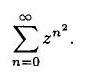
\includegraphics[max width=\textwidth]{2022_05_24_2551411173e3791eb07fg-23}

\begin{enumerate}
  \setcounter{enumi}{2}
  \item Suppose $f$ is analytic in the region $0<|z|<1$ and suppose there is a constant $K$ such that $|f(z)| \leq K|z|^{-\frac{1}{2}}$
\end{enumerate}
there. What kind of isolated singularity does $f$ have at zero? (Please prove your answer.)

\begin{enumerate}
  \setcounter{enumi}{3}
  \item For what values of $z$ does the series
\end{enumerate}
$$
\sum_{n=0}^{\infty} \frac{z^{n}}{1-z^{n}}
$$
converge? Is the sum an analytic function of $z$ ?

\begin{enumerate}
  \setcounter{enumi}{4}
  \item True-false: There is a non-constant entire function $f$ such $f(z+1)=f(z)$ and $f(z+i)=f(z)$ for all $z$ in $\mathbb{C}$.

  \item True-false: Suppose $\left\{f_{n}\right\}_{n=0}^{\infty}$ is a sequence of functions defined and analytic in the open unit disc, $|z|<1$. Suppose also that the values of each $f_{n}$ are contained in the upper half-plane, i.e., suppose that $\operatorname{Im}\left(\mathrm{f}_{\mathrm{n}}(\mathrm{z})\right) \geq 0$ for all $n$ and for all $z,|z|<1$. Then $\left\{f_{n}\right\}_{n=0}^{\infty}$ is a normal family.

\end{enumerate}
\section{Ph.D. Qualifying Examination in Analysis}
Professors Bor-Luh Lin and Paul S. Muhly

August 19, 2005

Instructions. Be sure to put your name on each booklet you use.

This examination is a true-false test. Each problem contains a statement that is either true or false. If you believe a statement is true, you must indicate so and give a proof. If you think it is false, you must indicate so and present a counter example.

The exam is divided into two parts. The first covers real analysis and the second covers complex analysis. Each part has 5 problems. You need only work 4 problems in each part. You must indicate which 4 you are submitting for evaluation. If you want to do five in a part, that is OK. We will treat the extra problem as a bonus.

\section{Part I}
\begin{enumerate}
  \item Let $f$ be a bounded measurable function on the interval $[0,1]$ and let $\epsilon>0$ be given. Then there is a step function $\sigma$ on $[0,1]$ such that $|f(x)-\sigma(x)|<\epsilon$ for all $x \in[0,1]$.

  \item If $\left\{f_{n}\right\}_{n \in \mathbb{N}}$ is a uniformly bounded sequence of nonnegative, Lebesgue integrable functions on $\mathbb{R}$ such that $\left\{f_{n}\right\}_{n \in \mathbb{N}}$ converges to zero pointwise on $\mathbb{R}$, then $\int_{\mathbb{R}} f_{n}(x) d x \rightarrow 0$.

  \item Suppose $\left\{f_{n}\right\}_{n \in \mathbb{N}}$ is a uniformly bounded sequence of Lebesgue measurable functions defined on [0,1] and for each $n \in \mathbb{N}$ and $x \in[0,1]$, let $F_{n}(x)=\int_{0}^{x} f_{n}(t) d t$. Then the sequence $\left\{F_{n}\right\}_{n \in \mathbb{N}}$ is equicontinuous on $[0,1]$.

  \item The composition of two absolutely continuous functions on $\mathbb{R}$ is absolutely continuous; i.e., if $f$ and $g$ are two absolutely continuous functions defined on $\mathbb{R}$, then $f \circ g$ is absolutely continuous.

  \item If $f$ is a continuous, non-decreasing function defined on $[0,1]$ and if $E \subseteq[0,1]$ is a set of Lebesgue measure zero, then $f(E)$ is a set of Lebesgue measure zero.

\end{enumerate}
\section{Part II}
\begin{enumerate}
  \setcounter{enumi}{6}
  \item The equation $\sin (z)=2$ has no solutions in the complex plane.

  \item Suppose $f$ is analytic in a region $G$ (in the complex plane) and that for some positive integer $n$, the $n^{t h}$ derivative of $f$ achieves its maximum modulus at a point $z_{0}$ in $G$. Then $f$ is a polynomial of degree at most $n$.

  \item Let $G$ be a region in the complex plane and let $z_{0}$ be a point in $G$. Suppose that $f$ is a function defined and analytic on $G \backslash\left\{z_{0}\right\}$ and that $f$ maps $G \backslash\left\{z_{0}\right\}$ into the upper half-plane. Then $z_{0}$ is a removable singularity of $f$.

  \item The function $f(z)=\csc (z)$ has a simple pole at $z=0$ and its residue there is 1 .

  \item Let $G$ be the open upper half-plane and for $z \in G$ define

\end{enumerate}
$$
\psi_{n}(z):=\exp \left\{\frac{i-(z-n)}{i+(z-n)}\right\},
$$
for $z \in G$ and $n \in \mathbb{N}$. Then $\left\{\psi_{n}\right\}_{n \in \mathbb{N}}$ is a normal family in $H(G)$ with no non-constant limit points.

\section{Ph.D. Qualifying Examination in Analysis}
January 9, 2019

Instructions. Be sure to put your name on each booklet you use.

This examination has a number of "true-false" questions in it. When a problem is a true-false problem, the operative statement will be preceded by True-False?. You are to decide whether it is true or false. If you think it is true, you must provide a proof. If you think it is false, you must provide a counter example or a proof of why it is false. No points will be given for a correct guess that the problem is true or false without any justification. Also, there will be no "Bankruptcy" points given.

The exam is divided into two parts. The first covers real analysis and the second covers complex analysis. Each part has 5 problems. You need only work 4 problems in each part. You must indicate which 4 you are submitting for evaluation. If you want to do five in a part, that is OK. We will treat the extra problem as a bonus, but still mark the four problems (in each part) that you think are your best work.

\section{Part I}
\begin{enumerate}
  \item Let $f$ be a real-valued continuous function mapping $[0,1]$ to $[0,1]$. True-False? $f$ is absolutely continuous if and only if $f$ maps Lebesgue null sets to Lebesgue null sets.

  \item Suppose $f$ is a non-negative Lebesgue integrable function defined on $[0,1]$. True-False? There is a Lebesgue measurable set $E \subseteq[0,1]$ such that $f=1_{E}$ if and only if $\int_{0}^{1} f^{n} d \mu=\int_{0}^{1} f d \mu$ for all positive integers $n$.

  \item For what values of $\alpha>0$ is the function $x \rightarrow x^{\alpha}$ absolutely continuous on every bounded subinterval of $[0, \infty)$ ?

  \item Let $\sigma$ be the function defined by the formula

\end{enumerate}
$$
\sigma(x):= \begin{cases}0, & x \leq 0 \\ 1, & x>0\end{cases}
$$
and let $\sigma^{*}$ be the outer measure determined by $\sigma$. True-False Every subset of $\mathbb{R}$ is measurable with respect to $\sigma^{*}$.

\begin{enumerate}
  \setcounter{enumi}{5}
  \item True-False The function
\end{enumerate}
$$
f(x):=\sum_{k=1}^{\infty} \sin (k x) / k^{m}
$$
is of bounded variation over every finite interval whenever $m>2$.

\section{Part II}
\begin{enumerate}
  \setcounter{enumi}{6}
  \item Suppose $f$ is holomorphic in the open unit disc $\mathbb{D}$. Suppose also that for each $z \in \mathbb{D}$ there is an integer $n(z)$ such that the derivative $f^{(n(z))}$ vanishes at $z$. True-False? $f$ must be a polynomial.

  \item True-False? There is a holomorphic function $f$ on the closed unit disc such that $f\left(\frac{1}{n}\right)=\frac{1}{n+2}, n \geq 1$.

  \item A function $f$ defined and analytic on a region $G$ is said to have a fixed point $z$ in $G$ if $f(z)=z$. If $f$ is analytic in a region that contains the closed unit disc and if $|f(z)|<1$ for all $z,|z|=1$, how many fixed points does $f$ have in the open unit disc?

  \item True-False? The function of $r$

\end{enumerate}
$$
\varphi(r):=\int_{|z|=r} \frac{\sin z}{z^{2}+1} d z, \quad r \neq 1
$$
can be extended to a continuous function defined on all of $[0, \infty)$. 10. Recall that a function $f$ defined on the extended complex plane $\widehat{\mathbf{C}}:=\mathbb{C} \cup\{\infty\}$ is said to be meromorphic on $\widehat{\mathbf{C}}$ in case $f$ is meromorphic on $\mathbb{C}$ and $f\left(\frac{1}{z}\right)$ has a non-essential singularity at $z=0$. Show that a nonconstant function that is meromorphic on $\widehat{\mathbb{C}}$ has the same number of zeros and poles in $\widehat{\mathbf{C}}$.

January 2020

\begin{abstract}
The exam has two parts: real analysis and complex analysis. Each part has five problems. Please solve any four problems in each part. 
 If you want to try the fifth problem in either part, the exam will be scored on the best four scores from each part.
\end{abstract}

Real Analysis. Solve any four problems from this group of five problems.

\begin{enumerate}
  \item Suppose $f_{n}(x), f(x)$ are functions in $L^{1}([0,1])$. Suppose $f_{n}(x) \rightarrow f(x)$ for every $x$, is it true that $\int_{(0,1)} f_{n}(x) d x \rightarrow \int_{(0,1)} f(x) d x ?$ Give a proof or a counterexample.

  \item Suppose $f \in L^{1}\left(R^{1}\right)$ is it true that $\lim _{x \rightarrow \infty} f(x)=0$ ? Give a proof or a counterexample.

  \item Suppose that a measurable set $E \subset(0,1)$ is such that $m(E \cap(r, s)) \geq$ $\frac{s-r}{4}$ for all rational $0<r<s<1$. Compute $m(E)$.

  \item Suppose $f_{k}, f$ are functions in $L^{2}([0,1])$ such that $f_{k}(x) \rightarrow f(x)$, a.e., and that $\left\|f_{k}\right\|_{L^{2}} \rightarrow\|f\|_{L^{2}}$. Is it true that $f_{k} \rightarrow f$ in $L^{2}$ ? Give a proof or a counterexample.

  \item Suppose $f$ is absolutely continuous and that $f^{\prime} \in L^{1}\left(R^{1}\right)$. Prove that $\lim _{x \rightarrow+\infty} f(x)$ exists. Does the limit have to be zero? Complex Analysis. Solve any four problems in this group of five problems.

  \item Find all entire functions $f$ for which there is a positive number $C$ such that $|f(z)| \leq C(1+|z|)$ for all $z$.

  \item Prove the uniform limit of a sequence of holomorphic functions is holomorphic.

  \item Suppose $f$ is holomorphic on the unit disc and satisfies the inequality $|f(z)| \leq(1-|z|)^{-1}$ for all $z$ in the disc. Prove that $\left|f^{\prime}(z)\right| \leq C(1-|z|)^{-2}$ for some constant $C$.

  \item Suppose $f$ is entire and that its imaginary part satisfies the inequality $\operatorname{Im}(f) \geq 0$. Show $f$ is a constant.

  \item Suppose $f$ is analytic in the annular region $1 \leq|z| \leq 2$. Suppose also that $|f| \leq 1$ on the circle $|z|=1$ and that $|f| \leq 4$ on the circle $|z|=2$. Show that $|f(z)| \leq|z|^{2}$ for all $z, 1 \leq|z| \leq 2$.

\end{enumerate}
\section*{Qualifying Exam -Analysis }
Summer 2017

\section{Rules of the exam}
\begin{itemize}
  \item You have 180 minutes to complete this exam.

  \item The exam contains a section of 4 problems in real analysis and a section of 4 problems in complex analysis. For maximum points you must submit solutions for 6 problems. Also you must attempt at least 2 problems in each section.

  \item Please mark the problems to be graded on the first column of the grading table on page $2 .$

  \item Show your work! - any answer without an explanation will get you zero points.

  \item Please read the questions carefully; some ask for more than one thing.

  \item Do not forget to write your name, see page 2 .

  \item You are not allowed to use a cell phone or a calculator during the exam.

\end{itemize}
\section{Good luck!}
\section{Real Analysis}
$\mathbf{R}$ - I: Solve at your choice ONE of the following problems:

a) Let $E$ be the subset of all elements in $[0,1]$ which do not contain the digits 3 and 9 in their decimal expansion. Is $E$ Lebesgue measurable? If yes find its measure.

b) Show that if $f: \mathbb{R} \rightarrow \mathbb{R}$ is measurable then the set $\left\{x \in \mathbb{R}: \mu\left(f^{-1}(x)\right)>0\right\}$ has measure zero.

$\mathbf{R}$ - II: Let $f_{n}:[-1,1] \rightarrow \mathbb{R}$ be a sequence of Lebesque measurable functions that converges to $f$ almost everywhere. If $\int_{[-1,1]}\left|f_{n}\right|^{4} d \mu \leq 1$ for every $n$ then show that $\int_{[-1,1]}\left|f_{n}-f\right| d \mu$ converges to 0 .

$\mathbf{R}$ - III: Let $(X, d)$ be a compact metric space and let $f: X \rightarrow X$ be a continuous function. Show that there exists $A \subseteq X$ a compact subset such that $f(A)=A$.

$\mathbf{R}$ - IV: Let $F_{k} \subset[0,1], k \in \mathbb{N}$ be measurable sets, and there exists $\delta>0$ such that $m\left(F_{k}\right) \geq \delta$ for all $k$. Assume the sequence $a_{k} \geq 0$ satisfies
$$
\sum_{k=1}^{\infty} a_{k} \chi_{F_{k}}(x)<\infty \text { for a.e. } x \in[0,1] \text {. }
$$
Show that
$$
\sum_{k=1}^{\infty} a_{k}<\infty
$$
Make sure you include all the details in your arguments.

\section{Complex analysis}
$\mathbf{C}-\mathbf{I}$ : Solve at your choice ONE of the following problems:

a) Compute the following integral
$$
\int_{-\infty}^{+\infty}\left(\frac{\sin x}{x}\right)^{3} d x
$$
b) Let $\mathcal{P}$ be the open region determined by the pentagon with vertices at $\omega^{k}$ where $k=\overline{0,4}$ and $\omega=\cos (2 \pi / 5)+i \sin (2 \pi / 5)$. Let $f: \overline{\mathcal{P}} \rightarrow \mathbb{C}$ be a continuous function that is analytic on $\mathcal{P}$. Assume that for every $t \in(0,1)$ we have that $\lim _{z \rightarrow \frac{2-t+t \omega}{2}} f(z)=\lim _{z \rightarrow \frac{2-t \omega^{2}+t \omega^{3}}{2}} f(z)=0$. Find $f$.

$\mathbf{C}$ - II: If we denote by $\mathcal{H}=\{z \in \mathbb{C}:|z-i|>1\}$ then describe all analytic, bijective maps $f: \mathcal{H} \rightarrow \mathcal{H}$.

$\mathbf{C}$ - III: Let $f$ be a non-constant, analytic function on the unit disk $\mathbb{D}$. If there exists a power series expansion $f(z)=\sum_{n=0}^{\infty} a_{n} z^{n}$ such that $\sum_{n=2}^{\infty} n\left|a_{n}\right| \leq\left|a_{1}\right|$ then show that $f$ is injective.

$\mathbf{C}$ - IV: Let $f$ be an analytic function on the open unit disk $\mathbb{D}$. Assume that for every $z \in(-1,0]$ the power series expansion around $z$ has a vanishing coefficient. Show that $f$ is a a polynomial function.

\section*{Ph.D. Qualifying Exam in Analysis, by Paul Muhly and Lihe Wang }
August 2019

\begin{abstract}
The exam has two parts: real analysis and complex analysis. Each part has five problems and solve any four problems from five problems in each part. 
 If you want to try the fifth problems, the exam will be graded as the best four scores from the five.
\end{abstract}

Real Variables. Solve any four problems in these five problems from real variables.

\begin{enumerate}
  \item Suppose $f_{n}(x), f(x)$ are measurable functions on $(0,1)$. Suppose $f_{n}(x) \rightarrow$ $f(x)$, it is true that $\int_{(0,1)} f_{n}(x) d x \rightarrow \int_{(0,1)} f(x) d x ?$ Give a proof or a counterexample.

  \item Suppose $f$ is a function defined $[0,1]$ and suppose that $|f(x)-f(y)| \leq$ $M|x-y|$ for all $x, y \in[0,1]$ where $M$ is a fixed constant. Prove that $f$ is differentiable a.e. and $\left|f^{\prime}(x)\right| \leq M$.

  \item Show that there is no measurable set such that that $m(E \cap(a, b))=\frac{b-a}{2}$ for all $a<b$, here $m(A)$ is the Lebesgue measure of $A$.

  \item Suppose $f_{k}, f$ are functions in $L^{1}([0,1])$ such that $f_{k}(x) \rightarrow f(x)$, a.e., and that $\left\|f_{k}\right\|_{L^{1}} \rightarrow\|f\|_{L^{1}}$. Then $f_{k} \rightarrow f$ in $L^{1}$.

  \item If $f \in L^{1}\left(R^{1}\right)$, show that $\sum_{n=-\infty}^{\infty} f(x+n)$ is convergent e.a to a function which has period $1 .$

\end{enumerate}
Complex Variables. Solve any four problems in these five problems from complex variables. 1. Find all entire functions with the condition that $|f(z)| \leq A\left(1+|z|^{2}\right)$ for some constant $A$.

\begin{enumerate}
  \setcounter{enumi}{2}
  \item Compute $\int_{\partial D(0,1)}(1+\bar{z})^{5} d z$.

  \item Suppose $f$ is holomorphic in the punctured disk $D(0,1) \backslash\{0\}$. Suppose also that $|f| \leq \frac{1}{|z|^{0.5}}$. Prove $f$ is differentiable at 0 .

  \item Suppose $f$ is entire so that $\operatorname{Re}(f) \geq 0$. Show $f$ is a constant.

  \item Suppose $f$ is holomorphic in the unit disk. Prove that there exists $z_{n}$ in the disk with $\left|z_{n}\right| \rightarrow 1$ that $f\left(z_{n}\right)$ is bounded.

\end{enumerate}
\section{Ph.D. Qualifying Examination in Analysis}
Professors Bor-Luh Lin and Paul S. Muhly

August 18, 2006

Instructions. Be sure to put your name on each booklet you use.

Much of this examination is "true-false". When a problem begins with "True-false", you are to decide if the operative assertion is true or false. If you decide that it is "true", you are to give a proof, while if you decide that it is "false", you are to present a counter example.

The exam is divided into two parts. The first covers real analysis and the second covers complex analysis. Each part has 5 problems. You need only work 4 problems in each part. You must indicate which 4 you are submitting for evaluation. If you want to do five in a part, that is OK. We will treat the extra problem as a bonus.

\section{Part I}
\begin{enumerate}
  \item True-false. Lebesgue measure is continuous in the sense that the Lebesgue measure of the closure of a set coincides with the Lebesgue measure of the set.

  \item True-false. Let $I_{1}$ and $I_{2}$ be two disjoint open intervals, and for $i=1,2$, let $A_{i}$ be an arbitrary subset of $I_{i}$. Then $m^{*}\left(A_{1} \cup A_{2}\right)=m^{*}\left(A_{1}\right)+m^{*}\left(A_{2}\right)$, where $m^{*}$ denotes Lebesgue outer measure.

  \item True-false. Let $\left\{f_{n}\right\}_{n \geq 0}$ be a sequence of non-negative integrable functions defined on $\mathbb{R}$ such that

\end{enumerate}
$$
0 \leq f_{1}(x) \leq f_{2}(x) \leq f_{3}(x) \leq \ldots
$$
and such that the sequence of numbers $\left\{\int_{\mathbb{R}} f_{n}(x) d x\right\}$ is bounded. Let $f(x)=\lim _{n \rightarrow \infty} f_{n}(x)$. Then $f(x)<\infty$ for almost all $x .$

\begin{enumerate}
  \setcounter{enumi}{4}
  \item True-false. Let $\sigma$ be the function on $\mathbb{R}$ that is zero to the left of $1,1 / 2$ for $1 \leq x<2,3 / 4$ for $2 \leq x<3$, $7 / 8$ for $3 \leq x<4$, etc. (Thus, $\sigma$ jumps by $2^{-n}$ at $n$ for $n=1,2, \ldots$, is constant between any two consecutive integers and is continuous from the right.) If $f(x)=x$ on $\mathbb{R}$, then $f$ is integrable with respect to the Lebesgue-Stieltjes measure determined by $\sigma$.

  \item Let $\left\{f_{n}\right\}$ be a uniformly bounded sequence of measurable functions defined on the interval $[0,1]$ and let

\end{enumerate}
$$
F_{n}(x)=\int_{0}^{x} f_{n}(t) d t \quad 0 \leq x \leq 1
$$
Show that there is a subsequence $\left\{F_{n_{k}}\right\}$ that converges uniformly on $[0,1]$.

\section{Part II}
\begin{enumerate}
  \item True-false. Suppose $f$ is analytic in the region $0<|z|<1$ and suppose that for each $r, 0<r<1$, the integral $\int_{C_{r}} f(z) d z=0$, where $C_{r}$ is the circle $|z|=r$. Then $f$ is analytic on the open unit disc.

  \item Suppose $f$ is analytic in the annular region $1-\epsilon<|z|<2+\epsilon$ for some positive $\epsilon$. Suppose also that $|f| \leq 1$ on the circle $|z|=1$ and that $|f| \leq 4$ on the circle $|z|=2$. Show that $|f(z)| \leq|z|^{2}$ for all $z$, $1<|z|<2$

  \item True-false. Let $\mathfrak{G}$ be a domain and let $z_{0}$ be a point in $\mathfrak{G}$. Suppose $f$ is analytic in $\mathfrak{G} /\left\{z_{0}\right\}$ and that $f$ takes values in the upper half-plane. Then $z_{0}$ is a removable singularity of $f$.

  \item Find the Laurent series representation of the function

\end{enumerate}
$$
f(z)=\frac{1}{z^{2}(1-z)}
$$
that is valid in the region $1<|z|<\infty$. 5. Let $f$ be analytic in the open unit disc $\mathbb{D}$ and let the Taylor series expansion for $f$ be
$$
f(z)=\sum_{n=0}^{\infty} a_{n} z^{n}
$$
Suppose\\
(a) $f(\mathbb{D}) \subseteq \mathbb{D}$\\
(b) $a_{0}=0$\\
(c) $\left|a_{1}\right|=1$

Calculate $\sup \left\{\left|a_{n}\right| \mid n \geq 2\right\}$.


\end{document}